\documentclass[11pt]{amsart}

\usepackage[utf8]{inputenc}
\usepackage{amsmath}
\usepackage{physics}
\usepackage{graphicx}

\renewcommand{\thesubsection}{\thesection.\alph{subsection}}

\title[Problem Sheet 4]{Hamiltonian Venture\\
	\hrulefill \small{ Problem Sheet 4: FYS3120 } \hrulefill}
	
\author[Winther-Larsen]{Sebastian G. Winther-Larsen}
\date{\today}

\begin{document}

\maketitle

\section{Constrained rod}

Figure \ref{fig:constrained_rod} shows a rod of lenth $b$ and evenly distributed mass $m$. One endpoint of the rod is constrained to move along a horizontal line, and the other endpoint is constrained to move along a vertical line. The two lines are in the same plane. There is no friction and the acceleration due to gravity is $g$.

\begin{figure}[ht]
\centering
	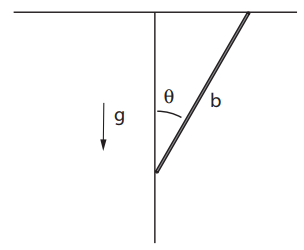
\includegraphics[width = 0.45\textwidth]{constrained_rod.png}
	\caption{Constrained rod}
	\label{fig:constrained_rod}
\end{figure}

\subsection{The Lagrangian and Lagrange's equation}
To fully describe the rod one needs one needs two translational coordinates and one rotational coordinate. The system has two constraints, so it is sufficient with one generalised coordinate, $\theta$, as the system only has one degree of freedom. The position of the left and right endpoint of the rod in terms of $\theta$ is
\begin{equation*}
(0, -b\cos \theta) \text{ and } (b\sin \theta, 0)
\end{equation*}
respectively. The position of the rods centre of mass must therefore be
\begin{equation}
\label{eq:com}
\vb{r} = (\frac{b}{2}\sin \theta, -\frac{b}{2}\cos \theta).
\end{equation}
It follows that 
\begin{equation*}
\dot{x} = \frac{b}{2}\dot{\theta}\cos \theta, \quad \dot{y} = \frac{b}{2}\dot{\theta}\sin \theta,
\end{equation*}
which gives
\begin{equation}
\label{eq:xandy}
\dot{x} + \dot{y} = \frac{b^2}{4}\dot{\theta}^2.
\end{equation}
The kinetic energy is the sum of translational and rotational energy\footnote{The moment of intertia for a rod rotating around its centre of mass is $I=\frac{mL^2}{12}$.}
\begin{equation}
\label{eq:travail1}
T 	= \frac{1}{2}m(\dot{x} + \dot{y}) + \frac{1}{2}I\dot{\theta}^2
	= \frac{1}{2}m\frac{b^2}{4}\dot{\theta}^2 + \frac{1}{2}\frac{mb^2}{12}
	= \frac{mb^2}{8}\dot{\theta}^2 + \frac{mb^2}{24}\dot{\theta}^2 
	= \frac{mb^2}{6}\dot{\theta}^2.
\end{equation}
The potential energy is
\begin{equation}
\label{eq:voltage1}
V 	= mgy = -\frac{1}{2}mg\cos \theta.
\end{equation}
The Lagrangian becomes
\begin{equation}
\label{eq:lagrangian1}
L = T - V = \frac{1}{6}mb^2\dot{\theta}^2 + \frac{1}{2}mgb \cos \theta 
\end{equation}

Lagrange's equation is given by
\begin{equation}
\label{eq:lagreqn}
\frac{d }{dt}\left(\frac{\partial L}{\partial \dot{\theta}} \right) - \frac{\partial L}{\partial \theta} = 0.
\end{equation}
Each part can be computed separately
\begin{align*}
\frac{\partial L}{\partial \theta} &= -\frac{1}{2} mgb \sin \theta \\
\frac{\partial L}{\partial \dot{\theta}} &= \frac{1}{3}mb^2\dot{\theta} \\
\frac{d }{dt}\left(\frac{\partial L}{\partial \dot{\theta}} \right) &= \frac{1}{3}mb^2 \ddot{\theta},
\end{align*}
and Lagrange's equation becomes
\begin{equation}
\frac{1}{3}mb^2\ddot{\theta} + \frac{1}{2}mgb \sin \theta = 0 \rightarrow 
\ddot{\theta} + \frac{3g}{2b}\sin \theta = 0
\end{equation}

\subsection{Equilibrium of the rod}
As usual, the system will tend towards a configuration where the potential, $V$, is as low as possible.  This point can be found by setting $\frac{\partial V}{\partial \theta} = 0$, but it is easy to see that it must be when $\theta = 0$.

When $\theta \to 0$, then $\sin \theta \to \theta$. Inserting this small-angle approximation into the Lagrange equation yields
\begin{equation}
\label{eq:lagapprox}
\ddot{\theta} + \frac{3g}{2b}\theta = 0,
\end{equation}
this equation corresponds to a harmonic oscillator with angular frequency $\omega = \sqrt{\frac{3g}{2b}}$. The period of an oscillation around the equilibrium orientation must then be
\begin{equation}
\label{eq:HOperiod}
T_0 = \frac{2\pi}{\omega} = 2\pi \sqrt{\frac{2b}{3g}}
\end{equation}

\section{Rotating pendulum}

\begin{figure}
\centering
	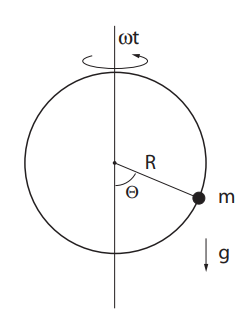
\includegraphics[width = 0.45\textwidth]{rotating_pendulum.png}
	\caption{Rotating pendulum}
	\label{fig:rotating_pendulum}
\end{figure}

\end{document}